% *******************************************************************************
% * Copyright (c) 2007 by Elexis
% * All rights reserved. This document and the accompanying materials
% * are made available under the terms of the Eclipse Public License v1.0
% * which accompanies this distribution, and is available at
% * http://www.eclipse.org/legal/epl-v10.html
% *
% *  $Id: einfuehrung.tex 4904 2009-01-03 17:58:33Z rgw_ch $
%
%*******************************************************************************
% !Mode:: "TeX:UTF-8" (encoding info for WinEdt)

\section{Introduction}
Dans Elexis les 'Views' (vue) sont les éléments centraux d'affichage et de contrôle.
Une 'View' affiche un certain genre de données de certaine manière et peut permettre un traitement définie de ces données. Les 'Views' peuvent être arrangées et sauvegardées selon vos besoins et habitudes de travail à ce qu'on appelle des perspectives. On peut aussi aménager à des différents postes de travail des différentes perspectives, puisqu'à l'accueil, dans le laboratoire et dans la chambre de consultation des travaux différents sont au premier plan.


Ainsi, contrairement à d'autres logiciels, chez Elexis l'interface utilisateur n'est pas définie par le fabricant, mais par l'utilisateur.

Dans ce chapitre, sont décrits les 'Views' qui sont comprises dans le système de base de Elexis.
Une telle énumération ne peut jamais être exhaustive, puisque des nouveaux Plugins (élaborés par nous ou d'autres) peuvent apporter à tout moment leurs propres 'Views'.
Celles-ci devraient alors être décrites dans la documentation du Plugin en question.


\subsection{Ouverture et fermeture d'une 'View'}
Tous les 'Views' existantes dans le système (aussi ceux qui sont apportés par les Plugins externes) sont accessibles par le menu fenêtre - affichage. Dans ce menu se trouvent parfois quelques 'Views' qui ont été arrangées pour la perspective actuelle, mais aussi toujours un point de menu  \glqq autres\ldots\grqq{}
respectivement \glqq Other\ldots\grqq{}. Ici on trouve une liste de tous les 'Views' groupées d'après des thèmes (cf Fig. \ref{fig:viewlist}).
%\usepackage{graphics} is needed for \includegraphics
\begin{figure}[htp]
\begin{center}
  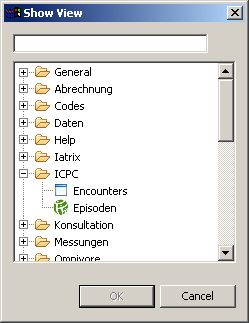
\includegraphics{images/showviewdialog}
  \caption{Liste aller Views}
  \label{fig:viewlist}
\end{center}
\end{figure}

Vous pouvez soit feuilleter cette liste, ou vous pouvez introduire en haut dans le champ de texte le nom de la 'View' cherchée. Aussitôt que vous commencez taper le nom,la liste sera filtré immédiatement selon les entrées existantes aux lettres correspondantes.

Marquez alors la 'View' de votre choix et ouvrez la soit par un double-clic soit en cliquant sur
\glqq OK\grqq{}.

\par
Pour fermer une 'View' il suffit de cliquer sur le symbole X dans l'onglet du fichier de la 'View' en question.

\subsection{Ouverture et sauvegarde d'une perspective}
\label{perspektiven} \index{perspective}
Une perspective est, comme expliqué en haut, une composition de 'Views' dotée d'un nom.
Elexis contient quelques perspectives prédéfinies qui sont accessibles par le menu démarrer respectivement par la barre d'outils. (Cf. aussi Fig. \ref{fig:toolbar}).

Une perspective a une importance spécifique en tant que  \glqq perspective de démarrage\grqq{}:
Cette perspective se présente toujours automatiquement après le login de l'utilisateur  correspondant sur le lieu de travail en question, ainsi que lorsqu'il clique sur le symbole 'Home' (ce bouton se trouve tout à gauche sur la barre d'outils). Toutes les autres perspectives (au choix de point de vue quantitative) peuvent être sauvegardées et accédées de nouveau sous un nom librement éligible. Les perspectives sont spécifiques au poste de travail. (Une perspective prête sur un lieu de travail n'est ainsi pas automatiquement disponible sur d'autres postes de travail) \footnote{Ceci doit être comme ça puisqu'il n'existent pas sur tout les postes de travail les mêmes Plugins - il n'est probablement pas indispensable que votre Plugin de comptabilité se trouve aussi sur le PC du laboratoire}.

\begin{itemize}
\index{perspective!perspective de démarrage}
\item Pour stocker l'arrangement 'View' actuel comme 'perspective de démarrage', choisissez sous  \textsc{fenêtre - perspective - sauvegarder comme perspective de démarrage}.

\item Pour sauvegarder la perspective actuelle à nouveau (p. ex. avec un arrangement ou une taille modifié de la 'View') choisissez le menu  \textsc{fenêtre - perspective - sauvegarder perspective.}.

\item Pour sauvegarder l'arrangement 'View' actuel sous un nom de perspective spécifique choisissez le menu \textsc{fenêtre - perspective - sauvegarder perspective sous …\ldots}

\item Pour restaurer la perspective actuelle (au cas où les changements apportés à la perspective ne conviennent pas ou si vous avez fermé par erreur des 'Views') choisissez  \textsc{fenêtre - perspective - restaurer}.

\item Pour revenir à la perspective de démarrage cliquez sur le symbole de la maison qui se trouve dans la barre d'outils tout à gauche.
\item Pour afficher une perspective sauvegardée choisissez 
\textsc{fenêtre - perspective - autres } et choisissez la perspective en question sur la liste. 

\end{itemize}
